\begin{figure}[htb]
  \centering
%segundo bloco de figuras
  \begin{tabular}{c c c }
    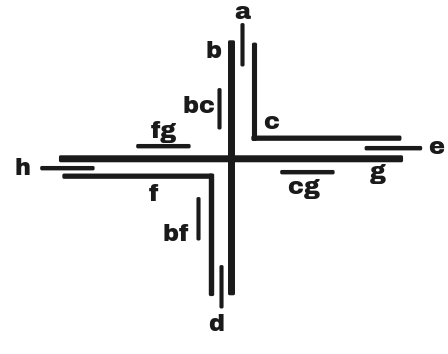
\includegraphics[width=4.5cm]{./img/falsePie.png}  %\label{fig:falsePie} 
    & &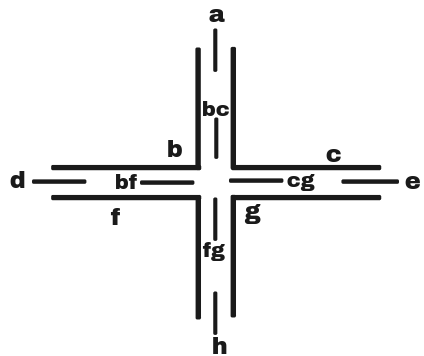
\includegraphics[width=4.5cm]{./img/truePie.png} %\label{fig:truePie}
    \\%[\abovecaptionskip]
    {\footnotesize (a) Baseado em torta falsa}  & &  {\footnotesize(b) Baseado em torta verdadeira}\\
  \end{tabular}
  \caption{Representação de dobra simples  de um dispositivo cláusula isomorfo ao grafo $H$} \label{fig:falseAndTruePie}
\end{figure} 